\chapter{Trout Recipes}

In this chapter we intend to publish Trout Recipes for dishes that have been 
attempted at Mbona. Please email your trout recipes to the editor at:

\href{mailto:hugh.murrell@gmail.com}{hugh.murrell@gmail.com}

Your recipe can be in plain text with an {\bf ingrediants} section
and an {\bf instructions} section. Please attach a photo of the resulting
dish just before eating commences. See our braai trout recipe for an example.

\clearpage


\section{Robertson's Braai Trout \\ (by Hugh Murrell)}

\subsection*{ingredients}

\begin{itemize}
\item 2 Whole Trout, gilled and gutted.
\item Robertsons Spice for Fish
\item 2 lemons
\item 1 Fennel Bulb
\item 1 lemon
\item For the Yogurt Dressing:
\begin{itemize}
\item 250ml Greek Yogurt, double cream
\item 45ml mayonnaise
\item 1 lemon, juiced
\item 10ml Wholegrain Mustard
\item Robertsons Coarsely Ground Black Pepper
\end{itemize}
\end{itemize}

\subsection*{instructions}

\begin{itemize}
\item Get your fire ready to braai the fish over medium hot coals.
\item Oil the inside of your grid to ensure that the fish doesn't stick to the grid.
\item Rinse the trout well under cold water, then pat dry with a tea towel.
\item Season the fish, inside and outside, with Robertsons Spice for Fish. 
\item Use lemon and sliced fennel slices to stuff into the cuts and cavity, 
then drizzle the stuffed parts with lemon juice. 
\item Place the fish inside a large hinged grid (without any foil) 
using a few lemon slices to protect the fish, see figure \ref{fig:braaiTroutPrepared}


 
\item braai over medium hot coals on both sides for about 30 minutes in total, see figure \ref{fig:braaiTroutPrepared}.


\item For the dressing, mix all the ingredients together.
\item Transfer the fish to a large serving platter and serve with a bowl of yogurt dressing, see figure \ref{fig:braaiTroutServed}

\end{itemize}

\subsection*{results}
  
\begin{figure}[H]
\centering
  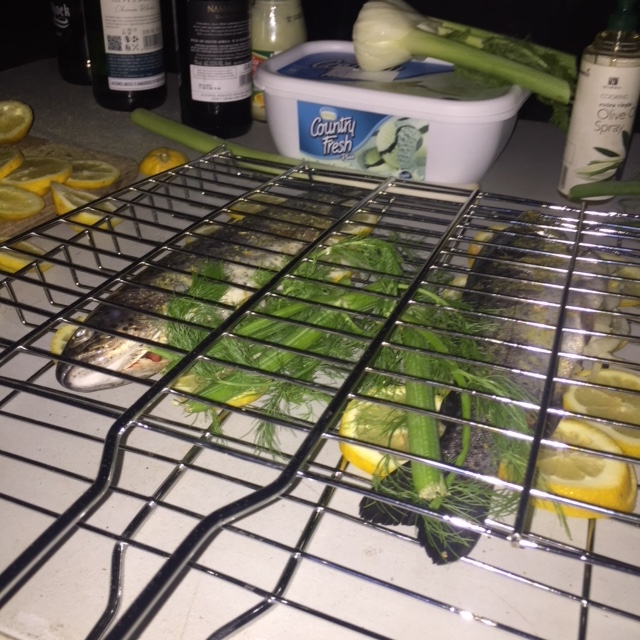
\includegraphics[scale=0.25]{recipes/braaiTroutPrepared.jpg} \hspace{1cm}  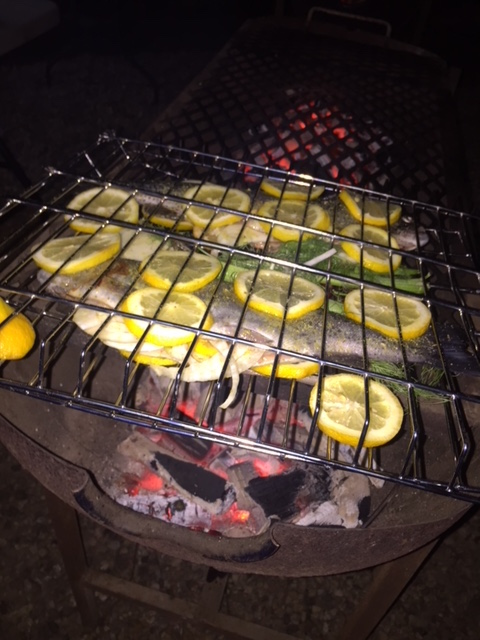
\includegraphics[scale=0.25]{recipes/braaiTroutCooking.jpg}
   \caption{Robertson's Braai Trout, prepared (left image) and on the coals (right image)}
  \label{fig:braaiTroutPrepared}
\end{figure}  


\begin{figure}[H]
\centering
  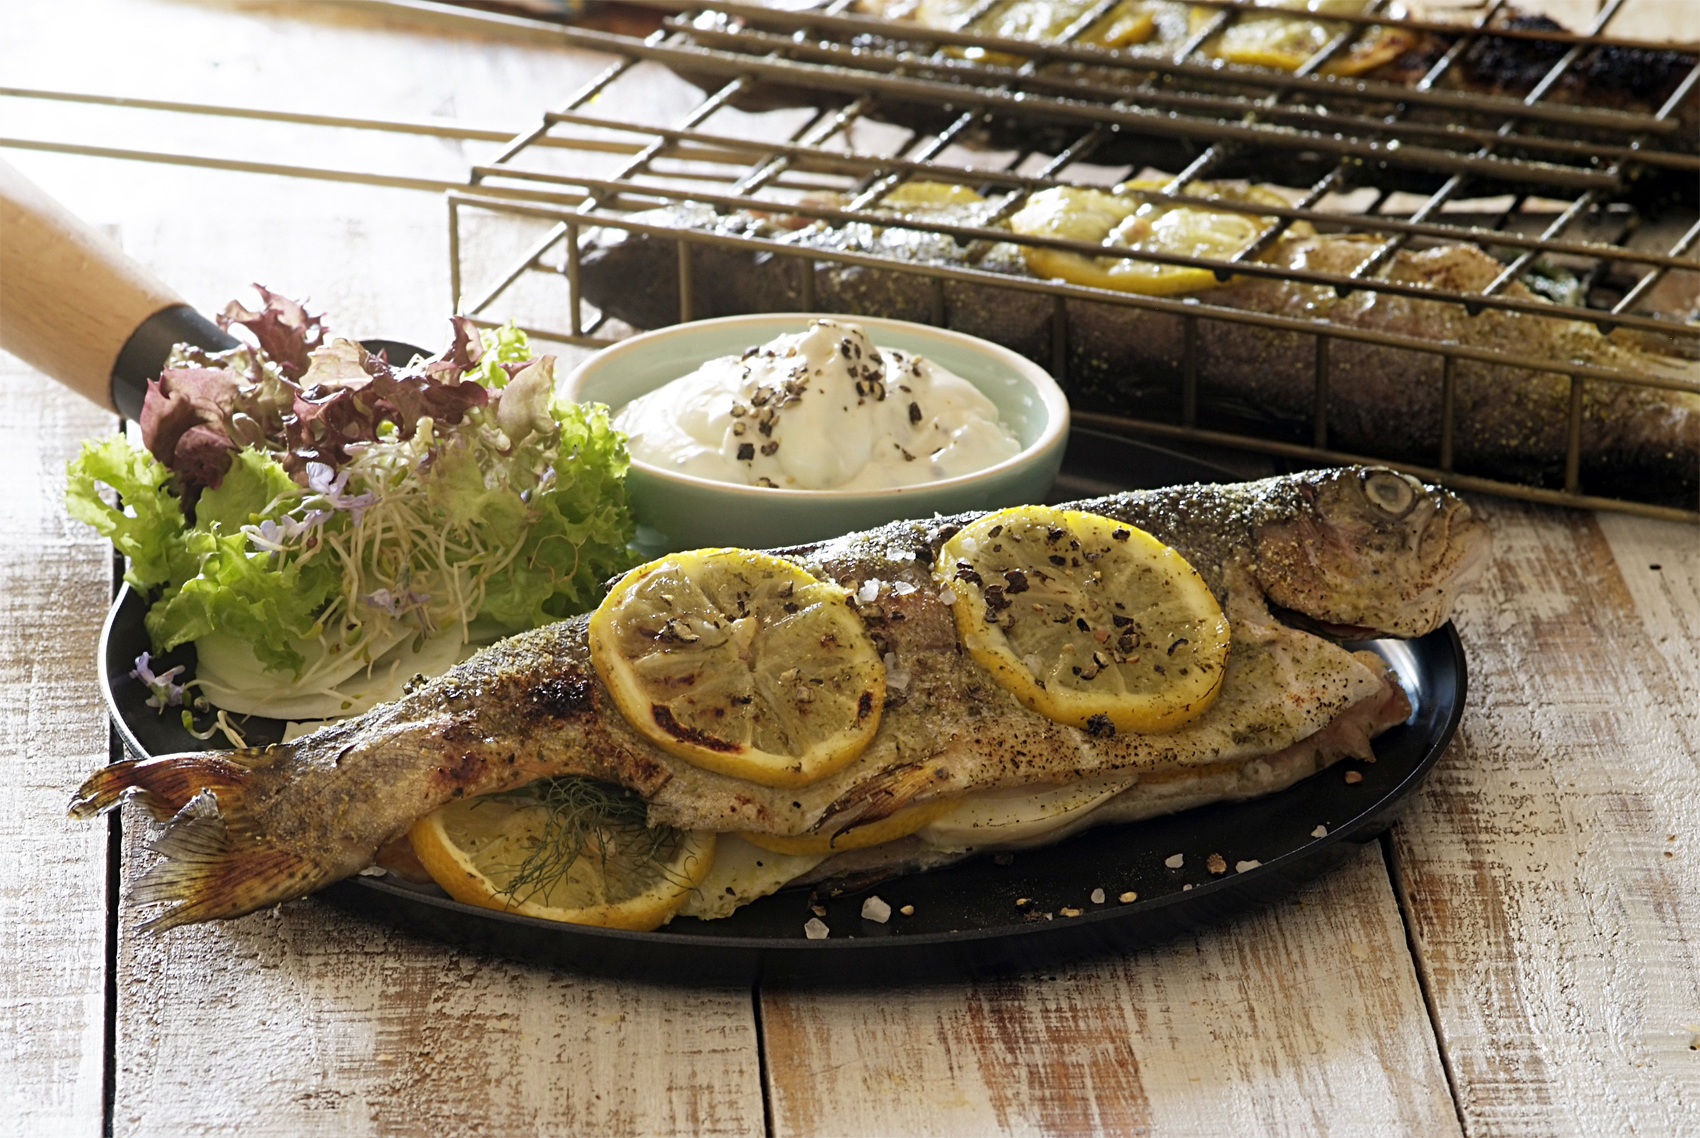
\includegraphics[scale=0.2]{recipes/braaiTroutServed.jpg}
   \caption{Robertson's Braai Trout, served and ready to be eaten.}
  \label{fig:braaiTroutServed}
\end{figure}


\section{Whole Baked Trout with Herb Salsa \\ (by Natasha Russo)} 

thanks to,  \url{http://eatdrinkpaleo.com.au/whole-baked-trout-recipe/}

\subsection*{ingredients for two trout}

\begin{itemize}
\item 2 Whole Trout, gilled, gutted and heads and tails removed.
\item For the salsa
	\begin{itemize}
		\item 1 medium red onion, peeled and roughly diced
		\item A handful of fresh basil leaves
		\item A handful of fresh parsley
		\item A few mint leaves
		\item 1 garlic clove, peeled
		\item Zest of 1 lemon
		\item Juice of half lemon 
		\item half cup olive oil
		\item 2 teaspoon sea salt
		\item half teaspoon black pepper
	\end{itemize}
\end{itemize}

\subsection*{instructions}

\begin{itemize}
	\item Preheat the oven to 200 centegrade
	\item Combine the salsa ingredients in a food processor or a blender and process into a salsa like consistency.
	\item Remove Heads and Tails and place the whole fish in a large roasting tray. 
	\item Cover the fish with the herb marinade on both sides and a little inside the fish cavity. 
	\item Bake in the oven for 20-25 minutes, on the middle shelf. 
	\item Remove and transfer to a platter or serve right in the roasting tray.
	\item Best with Spinach, Cranberry and Roast Almond Salad
\end{itemize}

\subsection*{results}
  
\begin{figure}[H]
\centering
  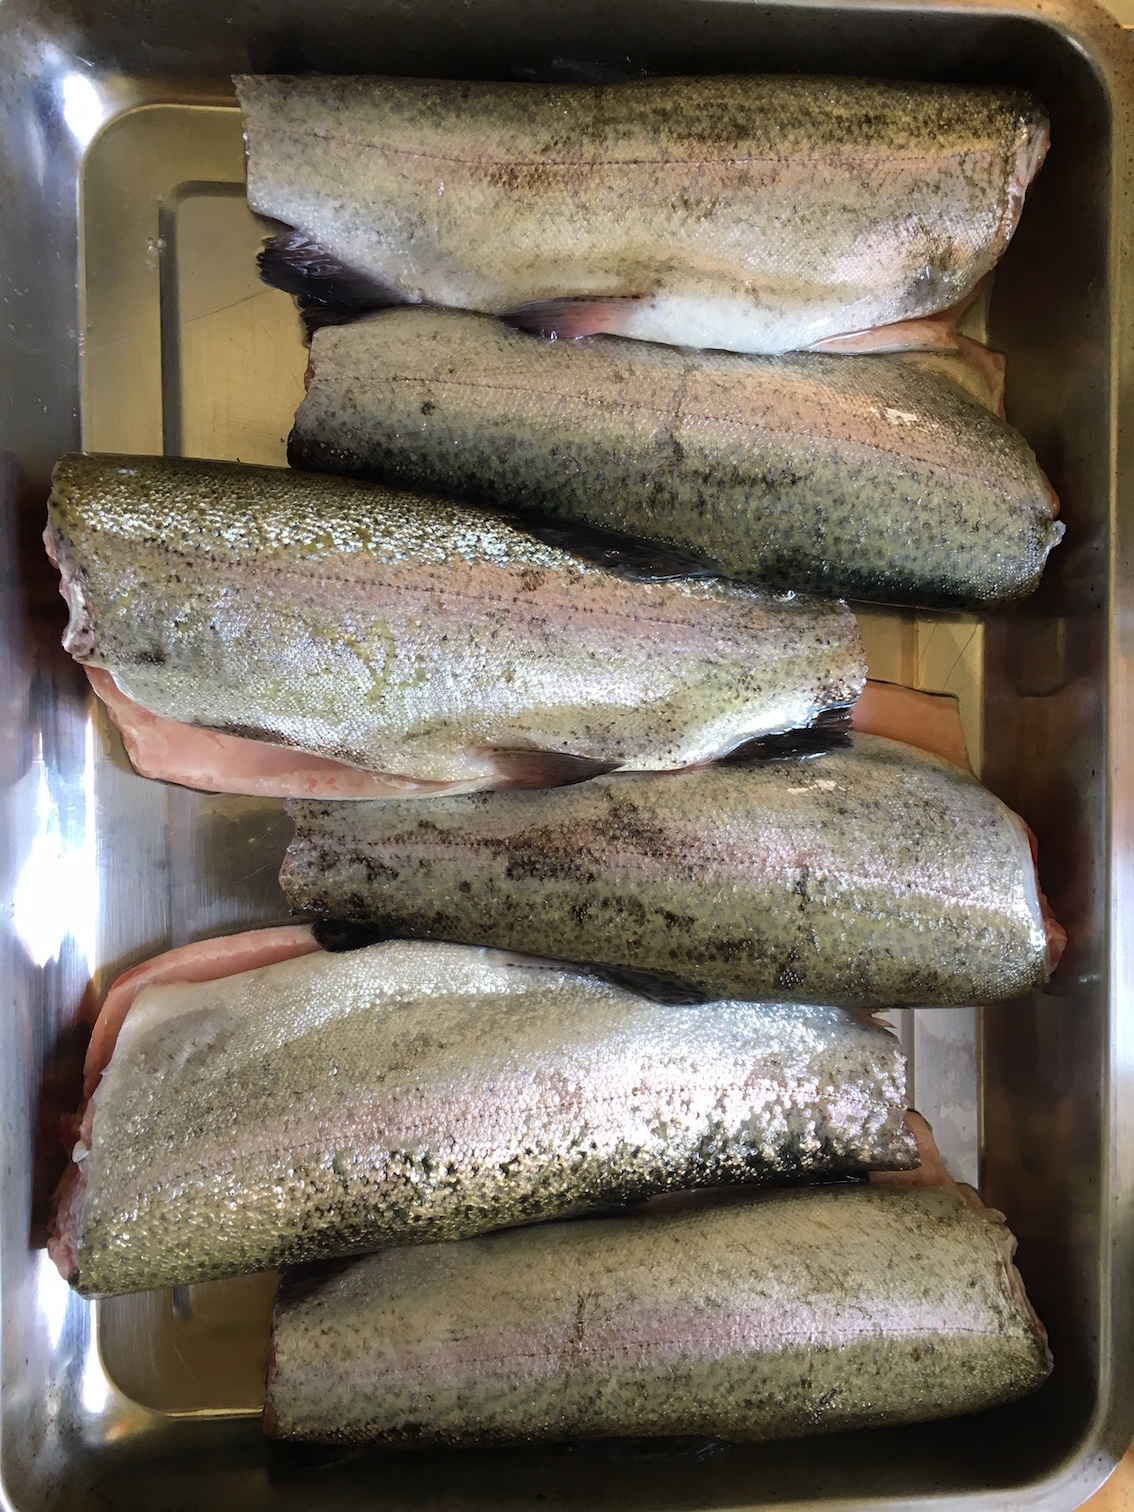
\includegraphics[scale=0.12]{recipes/NatashaPrepared.jpg} \hspace{1cm}  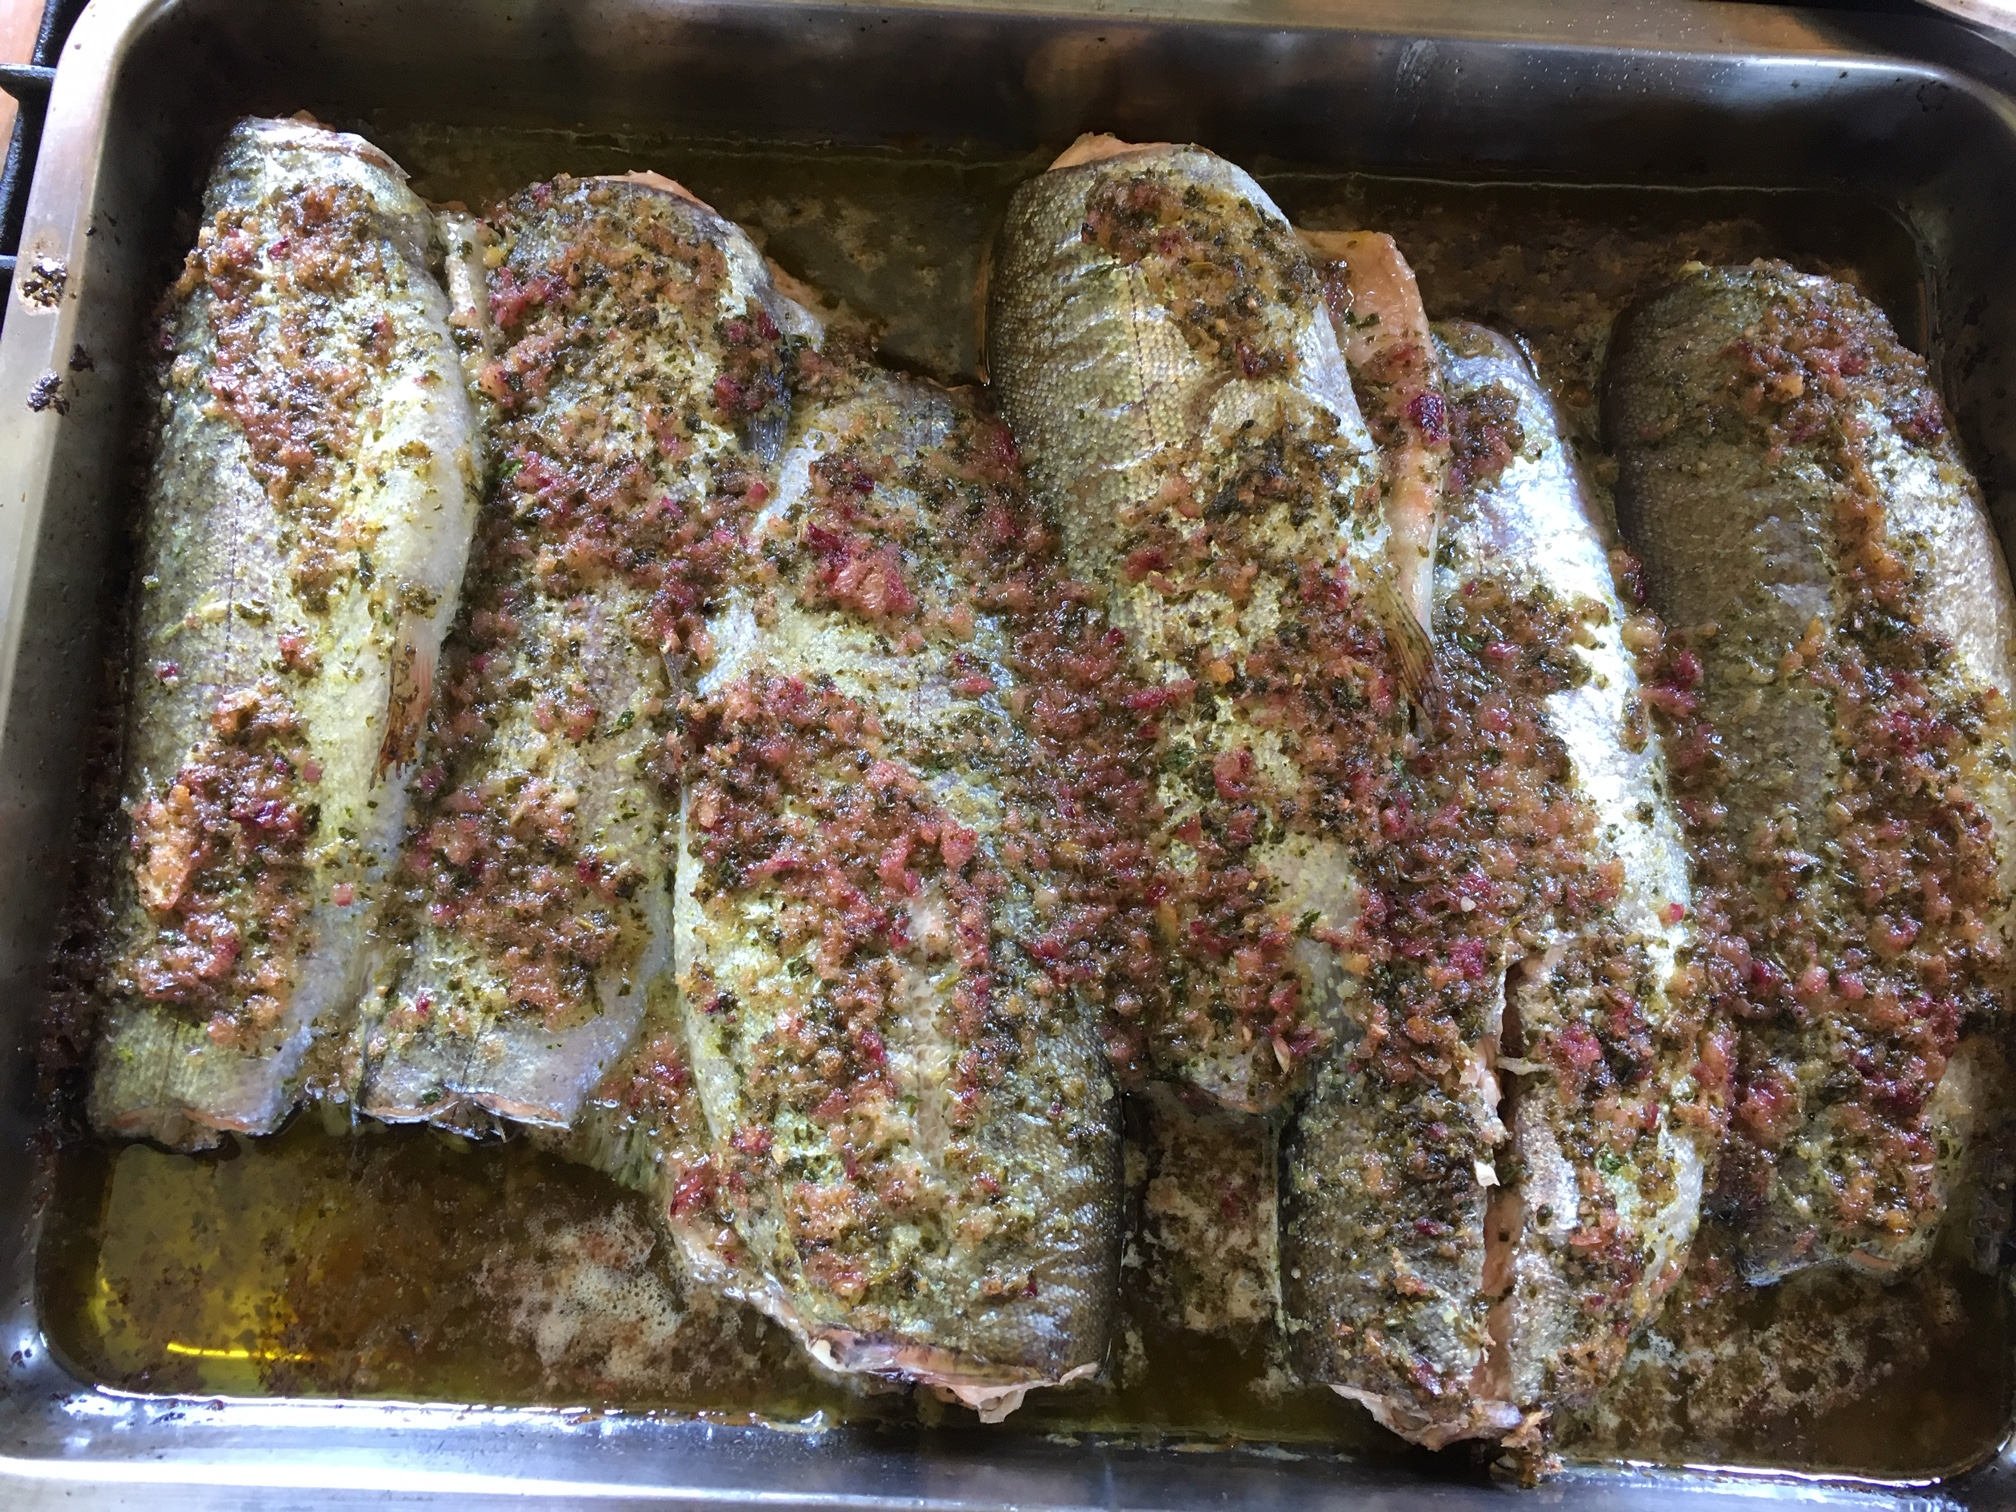
\includegraphics[scale=0.12]{recipes/NatashaPrecooked.jpg}
   \caption{Whole Trout, gutted (left image) and prepared (right image)}
  \label{fig:NatashaPrepared}
\end{figure}  

\begin{figure}[H]
\centering
  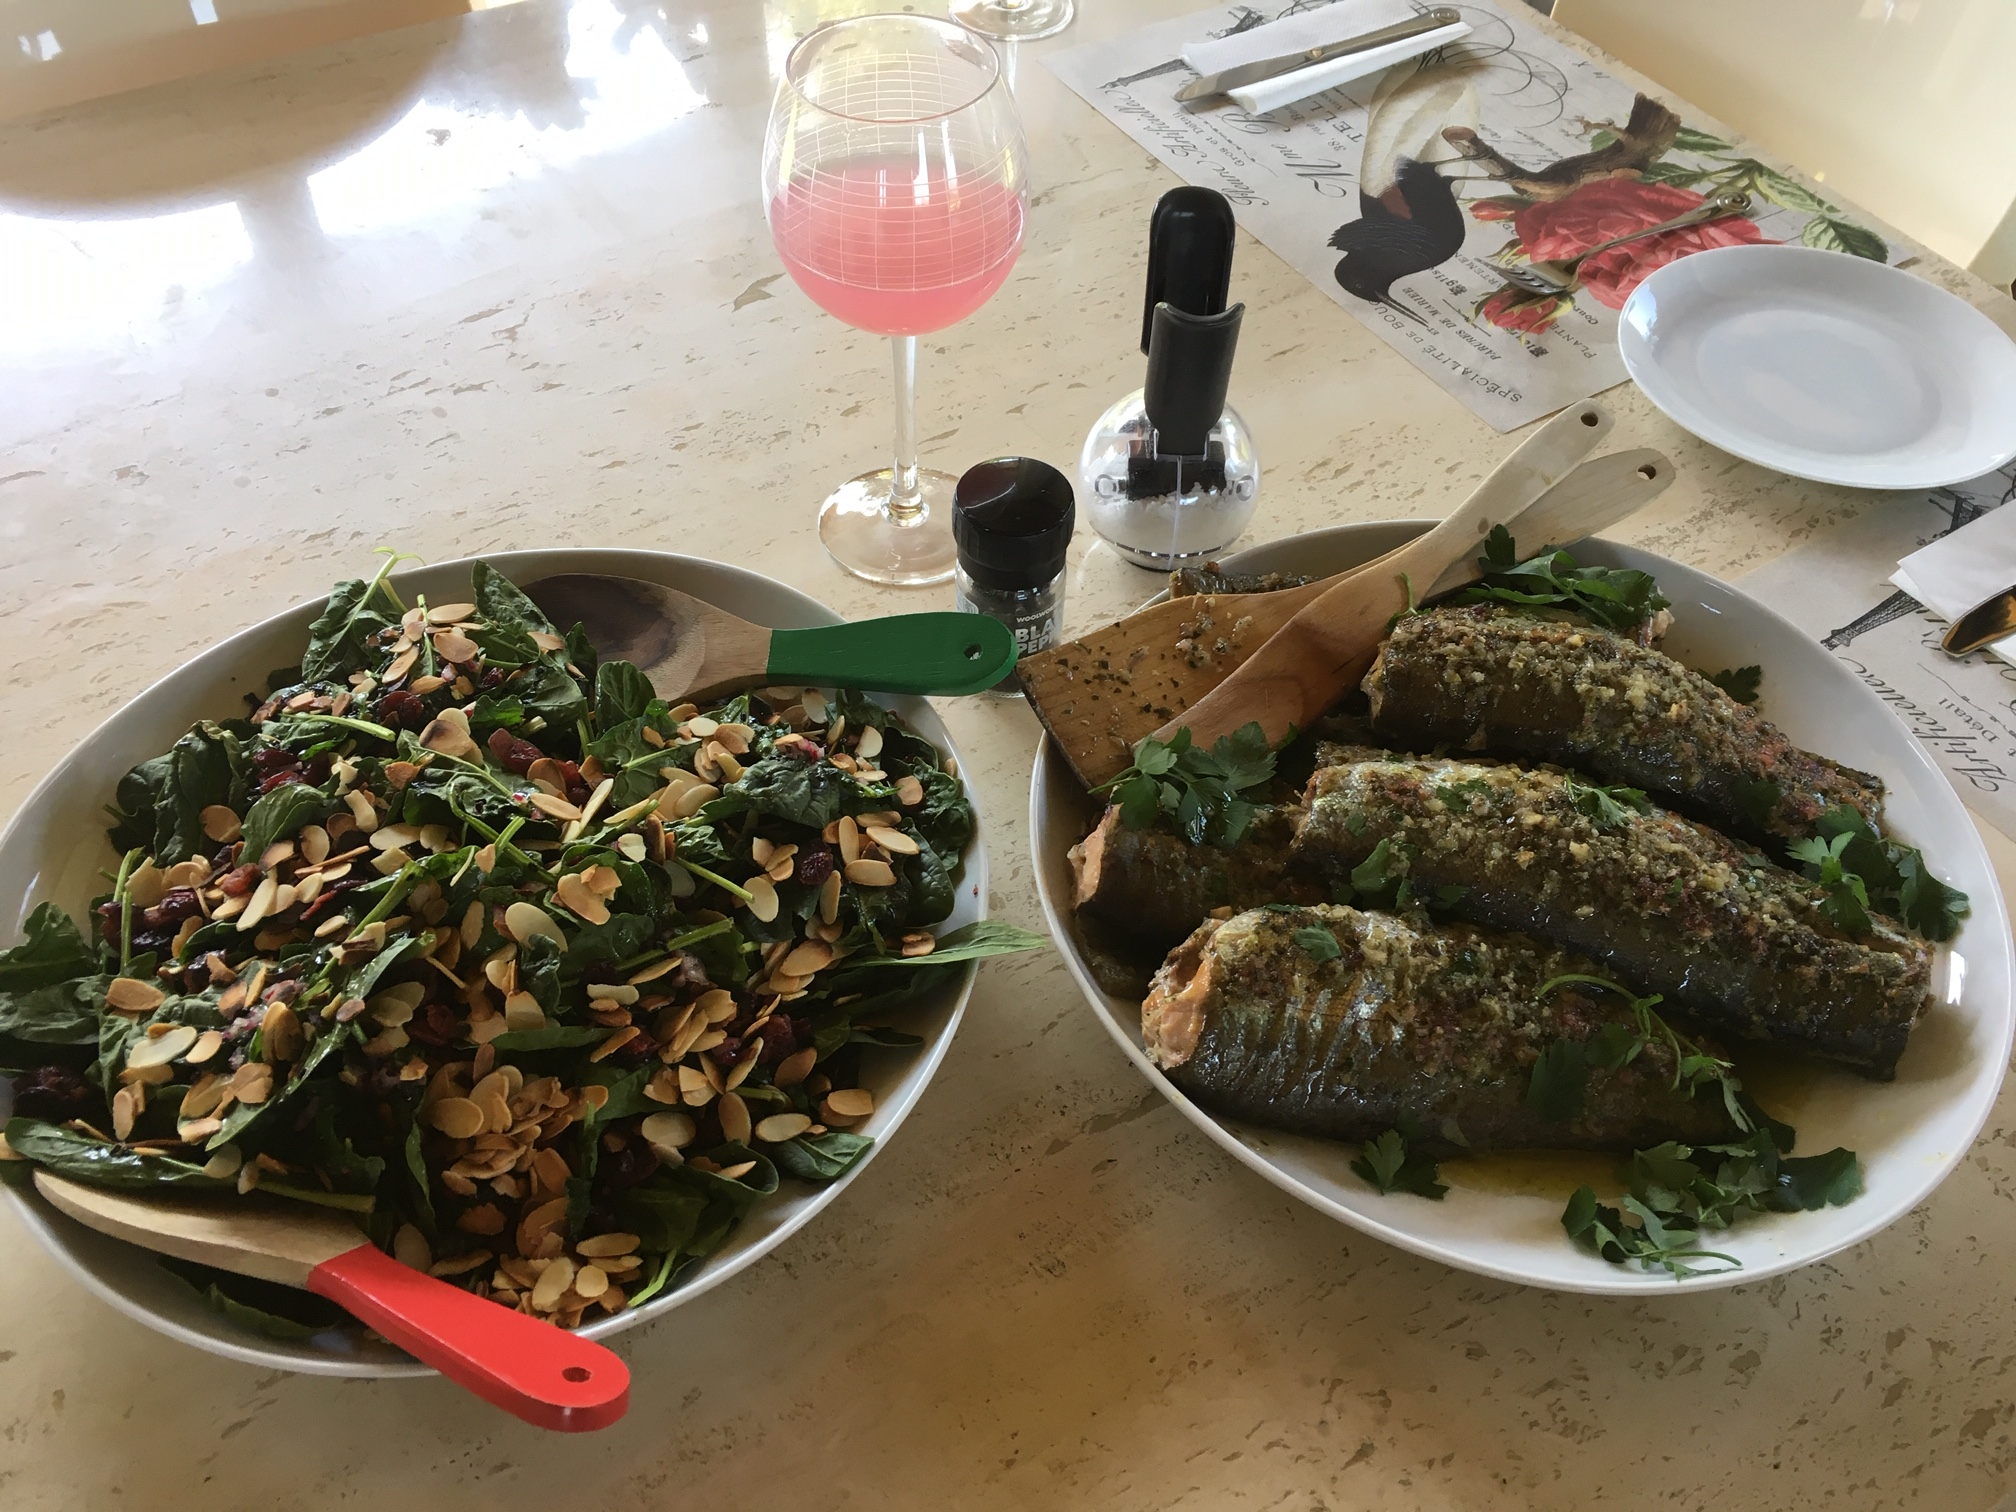
\includegraphics[scale=0.2]{recipes/NatashaServed.jpg}
   \caption{Natasha's Whole Baked Trout, served and ready to be eaten.}
  \label{fig:NatashaServed}
\end{figure}



